\documentclass[aspectratio=169,11pt]{beamer}

% Shared style (ib-tutorials.sty at the repo root).
\makeatletter\def\input@path{{./}{../}}\makeatother
\usepackage{ib-tutorials}

\usepackage[utf8]{inputenc}
\usepackage{amsmath,amssymb}
\usepackage{booktabs}
\usepackage{array}
\newcolumntype{L}[1]{>{\raggedright\arraybackslash}p{#1}}
\usepackage{graphicx}
\usepackage{xcolor}
\usepackage{listings}
\usepackage{tikz}
\usetikzlibrary{arrows.meta,positioning,shapes.geometric,fit,calc}
\usepackage{hyperref}

\newcommand{\sourcecredit}[1]{\vfill\hfill{\tiny\textcolor{DarkGray}{#1}}}

\lstset{
  basicstyle=\ttfamily\scriptsize\color{BlackGray},
  keywordstyle=\color{NavyBlue}\bfseries,
  commentstyle=\color{DarkGray}\itshape,
  stringstyle=\color{OliveGreen},
  showstringspaces=false,
  columns=fullflexible,
  keepspaces=true,
  frame=single,
  framerule=0.4pt,
  rulecolor=\color{LightGray},
  backgroundcolor=\color{LightGray!30},
  xleftmargin=0.25em,
  xrightmargin=0.25em
}
\lstdefinestyle{shell}{morecomment=[l]{\#}}

\title[Roadmap]{Roadmap and how to use}
\subtitle{The chapters, the software versions, and where the examples live}
\author[Miller]{Laura A. Miller}
\institute[UArizona]{Department of Mathematics, University of Arizona}
\date{Using IB Software \textbullet\ Part 0 \textbullet\ Chapter 0.2}

\newcommand{\partbox}[4]{\node[draw=#4,rounded corners=1pt,fill=#4!8,text width=#3,align=center,inner sep=2pt,font=\tiny] (#1) {\textbf{#2}};}

\begin{document}

% 1
\begin{frame}[plain]
\maketutorialtitlepanel{%
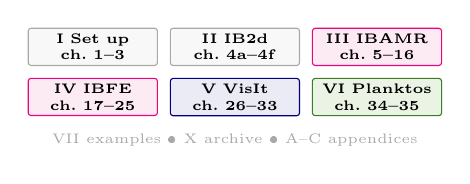
\begin{tikzpicture}[node distance=1.5mm and 1.5mm]
  \partbox{q1}{I Set up\\ch.\ 1--3}{15mm}{DarkGray}
  \node[draw=DarkGray,rounded corners=1pt,fill=DarkGray!8,text width=15mm,align=center,inner sep=2pt,font=\tiny,right=of q1] (q2) {\textbf{II IB2d\\ch.\ 4a--4f}};
  \node[draw=RubineRed,rounded corners=1pt,fill=RubineRed!8,text width=15mm,align=center,inner sep=2pt,font=\tiny,right=of q2] (q3) {\textbf{III IBAMR\\ch.\ 5--16}};
  \node[draw=RubineRed,rounded corners=1pt,fill=RubineRed!8,text width=15mm,align=center,inner sep=2pt,font=\tiny,below=of q1] (q4) {\textbf{IV IBFE\\ch.\ 17--25}};
  \node[draw=NavyBlue,rounded corners=1pt,fill=NavyBlue!8,text width=15mm,align=center,inner sep=2pt,font=\tiny,below=of q2] (q5) {\textbf{V VisIt\\ch.\ 26--33}};
  \node[draw=OliveGreen,rounded corners=1pt,fill=OliveGreen!8,text width=15mm,align=center,inner sep=2pt,font=\tiny,below=of q3] (q6) {\textbf{VI Planktos\\ch.\ 34--35}};
  \node[font=\tiny,text=DarkGray,below=1mm of q5] {VII examples \textbullet\ X archive \textbullet\ A--C appendices};
  %
\end{tikzpicture}}
\end{frame}

% 2
\begin{frame}{The parts and their chapters}
\scriptsize
\begin{tabular}{@{}L{0.03\textwidth}L{0.15\textwidth}L{0.74\textwidth}@{}}
\toprule
0 & Front matter & 0.1 About these notes \textbullet\ 0.2 this roadmap\\
I & Getting set up & 1 Computing on Puma \textbullet\ 1b Choosing software and building geometries \textbullet\ 2 Installing IBAMR with autoibamr \textbullet\ 3 Building and running an IBAMR application\\
II & IB2d & 4a Introduction and file formats \textbullet\ 4b the practical and VisIt for IB2d \textbullet\ 4c moving boundaries and your own example \textbullet\ 4d stability and convergence \textbullet\ 4e model gallery and muscle models \textbullet\ 4f meshes from images (MeshmerizeMe)\\
III & IBAMR fundamentals & 5 the IB method and numerical considerations \textbullet\ 6 structure files \textbullet\ 7 boundary conditions \textbullet\ 8a changing parameters, 8b non-dimensionalization \textbullet\ 9a target points, springs, several structures, 9b custom spring forces \textbullet\ 10 beams and curvature \textbullet\ 11 forces and output \textbullet\ 12 3D \textbullet\ 13 adding mass \textbullet\ 14 ConstraintIB \textbullet\ 15 IBAMR's own IB examples \textbullet\ 16 what can go wrong\\
IV & IBFE & 17 getting started \textbullet\ 18 creating meshes \textbullet\ 19 PK1 stress and body forces \textbullet\ 20 fiber tension and active stress \textbullet\ 21 two or more meshes \textbullet\ 22 3D flow past objects \textbullet\ 23 an IBFE main file, line by line \textbullet\ 24 advection--diffusion \textbullet\ 25 IBAMR's own IBFE examples\\
V & VisIt & 26 getting started \textbullet\ 27 3D \textbullet\ 28 Lagrangian and finite element data \textbullet\ 29 data analysis \textbullet\ 30 movies \textbullet\ 31 VisIt on the cluster \textbullet\ 32 the command line and Python \textbullet\ 33 converting and exporting data\\
VI & Planktos & 34 What is Planktos \textbullet\ 35 Using Planktos\\
VII & Examples guide & 36 catalogue of the examples, one page each\\
X & Archive (legacy) & X1 retired clusters and workflows \textbullet\ X2 old install recipes \textbullet\ X3 old IBAMR and libMesh code mapped to current code \textbullet\ X4 course logistics\\
A--C & Appendices & A MATLAB and Python helper codes \textbullet\ B glossary, references and credits \textbullet\ C exercises and homework\\
\bottomrule
\end{tabular}
\par\scriptsize Chapters are added to the repository as they are written; the table in the README says which exist.
\end{frame}

% 3
\begin{frame}{Suggested paths}
\begin{columns}[T,onlytextwidth]
\begin{column}{0.5\textwidth}
\begin{itemize}
  \item \al{A first simulation on the cluster, in a week:} 1 $\to$ 2 $\to$ 3 $\to$ example IB/01 $\to$ 26.
  \item \al{No cluster, no C++ (IB2d on your laptop):} 4a $\to$ 4b $\to$ 4c, then 4d--4f.
  \item \al{The IBAMR track:} 3 $\to$ 5 $\to$ 6 $\to$ 7 $\to$ 8a $\to$ 9a $\to$ 10 $\to$ 11 $\to$ 16, with 12--15 as needed.
  \item \al{The IBFE track:} 17 $\to$ 18 $\to$ 19 $\to$ 20 $\to$ 21 $\to$ 22 $\to$ 23 $\to$ 24, then 25.
  \item \al{Visualization and analysis:} 26 $\to$ 27 $\to$ 28 $\to$ 29, then 30--33.
  \item \al{Organisms in simulated flows:} 34 $\to$ 35.
\end{itemize}
\end{column}
\begin{column}{0.47\textwidth}
\begin{punchbox}
\small Every chapter can be read on its own. Where a chapter needs something from an earlier one, the slide says so.
\end{punchbox}
\vspace{2mm}
\small \textbf{Instructors:} Appendix C collects the exercises and homework from the courses (problems only). The example READMEs' ``Things to try'' sections make short labs.
\vspace{2mm}

\small \textbf{If you taught with the older notes:} each chapter ends with a slide ``What changed since the older course notes'', and Part X keeps the retired material.
\end{column}
\end{columns}
\end{frame}

% 4
\begin{frame}{Software versions used in these notes}
\scriptsize
\begin{tabular}{@{}L{0.18\textwidth}L{0.76\textwidth}@{}}
\toprule
IBAMR & \al{0.16.0} (31 January 2025), the version installed on Puma, and \al{0.19.0} (11 March 2026), the latest release. Every example was built and run with both, except IB/13 and the three ConstraintIB examples, run with 0.19.0 (chapter 36). 0.19.0 writes the velocity only as the vector \code{U}; older versions also wrote \code{U\_x}, \code{U\_y}, \code{U\_z}.\\
IBAMR 0.20 (in development) & drops the autotools build: only CMake remains. Everything here builds with CMake and starts with \code{IBTKInit}, so it is ready for 0.20.\\
autoibamr & the installer used in chapter 2 (commit \code{9c1e0a5}, October 2026), which pins libMesh 1.7.8 and PETSc 3.23.3 for these IBAMR versions.\\
Compilers and MPI & GCC 13.3 and Open MPI 4.1.6 on Ubuntu 24.04 (also under WSL2 on Windows); on Puma the modules \code{gnu13} and \code{openmpi5}.\\
IB2d & the GitHub version cloned on 6 March 2024 (commit \code{58663e1}; chapters 4a--4f), in MATLAB R2024a or Python 3.12 (pyIB2d, with the tracer fix of chapter 4b).\\
VisIt & 3.5.0.\\
gmsh & 4.12.1 (meshes in MSH 2.2 text format); Coreform Cubit for hexahedral meshes.\\
Planktos & 1.0.3, commit \code{a1c2128} (19 August 2026), in Python 3.12 (chapters 34 and 35).\\
Helper scripts & MATLAB R2024a; every MATLAB script has a Python 3 version, checked against Octave 8.4: 26 scripts outside \code{examples/legacy} (Appendix A).\\
\bottomrule
\end{tabular}
\vspace{2mm}
\begin{punchbox}
\small When a newer IBAMR appears, the chapter-3 porting checklist and the example READMEs say what to check first: the build (CMake), the input keys, and the output variable names.
\end{punchbox}
\end{frame}

% 5
\begin{frame}[fragile]{Where the examples live (1/2): the tree}
\label{fr:tree}
\begin{columns}[T,onlytextwidth]
\begin{column}{0.48\textwidth}
\begin{lstlisting}[style=shell,basicstyle=\ttfamily\tiny\color{BlackGray}]
examples/
  IB/      01-rubber-band         (ch. 3, 6)
           02-pulsatile-channel   (ch. 7)
           03-tethered-beam       (ch. 7, 10)
           04-moving-cylinders    (ch. 9a)
           06-growing-springs     (ch. 9a)
           07-moving-plates       (ch. 9a)
           08-glycocalyx-3d       (ch. 12)
           09-curling-beam        (ch. 10)
           10-jellyfish-bell      (ch. 10)
           11-heart-tube-pump     (ch. 9b)
           12-spider-ballooning   (ch. 13)
           13-carotid-bifurcation (ch. 7, 25, 26)
\end{lstlisting}
\end{column}
\begin{column}{0.5\textwidth}
\begin{lstlisting}[style=shell,basicstyle=\ttfamily\tiny\color{BlackGray}]
  IBFE/    01-tethered-plate      (ch. 17)
           05-gmsh-triangle       (ch. 18)
           06-active-tension      (ch. 20)
           08-plate-hits-circle   (ch. 21)
           10-flow-tank-plate-3d  (ch. 22)
           12-advection-diffusion (ch. 24)
  ConstraintIB/  01, 02, 03       (ch. 14)
  IB2d/      six folders          (ch. 4c-4f)
  analysis/  readers, VisIt scripts (ch. 11, 27-35)
  Planktos/  agents in these flows  (ch. 34, 35)
  support/   matlab-exercises     (App. A)
  legacy/    the course codes as they were
\end{lstlisting}
\end{column}
\end{columns}
\vspace{1mm}
\small There is no IB/05 in the public repository. Chapter 36 has one page per example.
\end{frame}

\begin{frame}{Where the examples live (2/2): what every folder holds}
\label{fr:folders}
\small Every example folder holds
\begin{itemize}
  \item \code{main.cpp}, the IBAMR program, and \code{CMakeLists.txt} to build it; \code{input2d} or \code{input3d}, with Unix line endings; \code{job.slurm} for Puma;
  \item the structure files (\code{.vertex}, \code{.spring}, \ldots) or the mesh, and the MATLAB and Python scripts that make them;
  \item \code{README.md}: what the example shows, how to build and run it, \al{what you should see}, how to look at it in VisIt, things to try, and its history.
\end{itemize}
\begin{punchbox}
\small Chapter 36 is the catalogue, one page per example. The numbers in the READMEs were measured with the shipped files; if yours differ, something in your set-up is different.
\end{punchbox}
\end{frame}

% 6
\begin{frame}[fragile]{Getting the notes and compiling the decks}
\begin{columns}[T,onlytextwidth]
\begin{column}{0.5\textwidth}
\begin{lstlisting}[style=shell,basicstyle=\ttfamily\tiny\color{BlackGray}]
git clone \
  https://github.com/fairyflies9/Using-IB-Software.git
cd Using-IB-Software/1-Getting-Set-Up
pdflatex 3-Building-and-Running-IBAMR.tex
\end{lstlisting}
\begin{itemize}
  \item Each chapter compiles on its own with \code{pdflatex} (TeX Live 2024 or newer), from its folder or from the repository root.
  \item The shared style is \code{ib-tutorials.sty} at the root; the decks find it through \code{\textbackslash input@path}. The figures are in \code{pictures/}.
  \item The PDFs are committed next to the sources, so you need not compile anything to read them.
\end{itemize}
\end{column}
\begin{column}{0.47\textwidth}
\begin{itemize}
  \item A combined PDF of all chapters, with a table of contents, will be added when the chapters are complete.
  \item While the series is being written it lives on the branch \code{master-tutorial}; \code{main} keeps the original lectures until the new version is reviewed.
  \item The theory series is also on Overleaf; these notes are not.
\end{itemize}
\begin{homebox}
\small Clone the repository now: the examples in Part I assume it is at \code{\textasciitilde/Using-IB-Software} on Puma.
\end{homebox}
\end{column}
\end{columns}
\end{frame}

% 7
\begin{frame}{Conventions in the slides}
\begin{columns}[T,onlytextwidth]
\begin{column}{0.5\textwidth}
\begin{itemize}
  \item \al{Red} marks the point of a slide or the thing most often done wrong.
  \item \code{Typewriter text} is something you type, a file name, or an input key, exactly as spelled; it can be copied from the PDF.
  \item Listings show commands (\code{\$} is not typed) and the \emph{exact} text of error messages.
  \item A gray box is the take-away; a pink box is what to do next.
  \item \emph{Legacy} marks something from the older notes that still works but is no longer the recommended way.
\end{itemize}
\end{column}
\begin{column}{0.47\textwidth}
\begin{itemize}
  \item Units: the IB examples use SI units (m, s, kg); the IBFE examples are dimensionless. Chapter 8b explains how to move between them.
  \item $\Delta x$ is the spacing of the finest grid level; \code{DT} is the time step as the input file calls it; $N$ is the number of cells across the coarsest level.
  \item ``Puma'' is the University of Arizona cluster (chapter 1). Everything also runs on a laptop with Linux, macOS, or Windows with WSL2 (chapter 2).
  \item References to the theory series look like \emph{Theory, module 3}.
\end{itemize}
\end{column}
\end{columns}
\end{frame}

% 8
\begin{frame}{Summary}
\begin{enumerate}
  \item Parts I--VII cover set-up, IB2d, IBAMR, IBFE, VisIt, Planktos and the examples; Part X is the archive; A--C are the appendices.
  \item Pick a path: first simulation, IB2d only, IBAMR, IBFE, visualization, or Planktos.
  \item The code targets IBAMR 0.16.0 and 0.19.0 with CMake, and is ready for 0.20.
  \item The examples are in \code{examples/IB}, \code{IBFE}, \code{ConstraintIB} and \code{IB2d}, with \code{analysis}, \code{Planktos} and \code{support} beside them, each with a README that says what you should see (chapter 36).
  \item Clone the repository; every deck compiles with \code{pdflatex}, and the PDFs are already there.
\end{enumerate}
\vspace{3mm}
\begin{homebox}
\small Next, Part I: chapter 1 (computing on Puma), chapter 1b (choosing software and building geometries), chapter 2 (installing IBAMR), chapter 3 (building and running).
\end{homebox}
\end{frame}

\end{document}
